\documentclass{article}
\usepackage[utf8]{inputenc}
\usepackage{geometry}
\usepackage{fancyhdr}
\usepackage{amsmath}
\usepackage{graphicx}
\usepackage{hyperref}

% Title Info
\title{Want2Remember SDD}
\author{CS3338 Group 3: Joshua Hanscom, Nicholas Montales, Jessie Guijosa, Perla Reyes}
\date{20 November 2024}

% Page Layout
\geometry{a4paper, margin=1in}
\pagestyle{fancy}
\fancyhead[R]{Page \thepage}
\fancyfoot[R]{SDD}

\begin{document}
\maketitle
\newpage
\tableofcontents
\newpage

\section*{Version Description}
\begin{tabular}{|c|p{10cm}|c|}
\hline
\textbf{Version} & \textbf{Description of Changes} & \textbf{Date} \\ \hline
1.0 & Initial version of the Software Design Document. & 20 November 2024 \\ \hline
1.1 & Snapshot 1: Memory Home Page & 9 December 2024 \\ \hline
1.2 & Snapshot 2: Memory Creation Page & 9 December 2024 \\ \hline
1.3 & Snapshot 3: More Details Page & 10 December 2024 \\ \hline
1.4 & Snapshot 4: Memory Contact Page & 10 December 2024 \\ \hline
\end{tabular}
\newpage

\section{Introduction}
\subsection{Purpose of the Document}
Want2Remember is a web application that assists those with cognitive impairments in remembering day-to-day tasks and memories. The system keeps track of user-generated data, such as memories, to-do lists, appointments, contacts, and payment information. This document explains the functionality, design, architecture, and requirements of the Want2Remember application.

\subsection{Intended Audience}
This document is intended for the California State University of Los Angeles (CSULA) Computer Science department. It is part of the Senior Design Project sponsored by We2Link. The audience includes professors, students of CSULA, and employees of We2Link.

\subsection{Overview of the System}
Want2Remember uses a component-based architecture to enhance reusability and reduce the size and complexity of the codebase.

\section{System Architecture}
\subsection{Workflow of the System}
The Want2Remember app allows users to store and create memories while enabling caregivers to provide support. User data is stored in Firebase. Users can create and edit memories, which are synchronized in real-time with Firebase. Caregivers can also interact with the app to assist users.

\begin{figure}[h!]
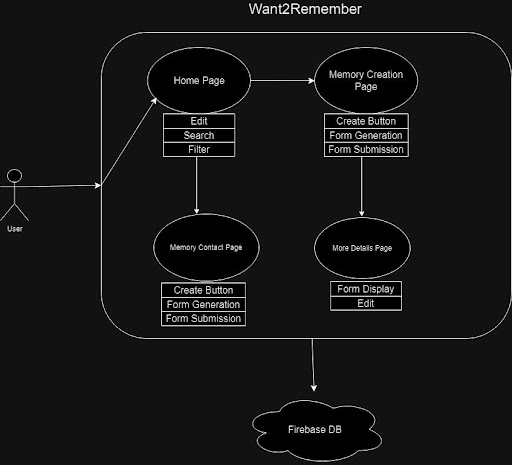
\includegraphics[width=0.5\textwidth]{snapshot4img4.jpg}
\caption{Workflow}
\end{figure}

\subsection{System Components}
\textbf{Client-Side:} 
The client side uses React for the web interface and React Native for the mobile app. Tailwind CSS ensures responsive and consistent styling. Key screens include:
\begin{description}
\item[Caregivers screen:] Displays caregiver information and access.
\item[Memories Creation Page:] Allows the user to create Memory tiles in order to save information that they could forget. There should also be a longer description that can be attached to every memory tile. The information should also be able to be viewed by clicking the memory tile.
\item[Contact Memory Creation Page:] Allows the user to create Memory tiles in order to save contact information that they could forget. There should also be a longer description that can be attached to every contact memory tile. The information should also be able to be viewed by clicking the contact memory tile.
\item[Account screen:] Allows users to manage settings.
\end{description} details (e.g., category, date, location).

\textbf{Server-Side:} 
Firebase serves as the backend, providing real-time data storage and synchronization. Firebase Authentication ensures secure user access. React JS components handle interactions with Firebase, ensuring seamless updates.

\section{User Interface}
\subsection{How to Use the System}
Users interact through various screens, including login, dashboard, and memory creation. Real-time data updates are stored in Firestore. Features include filtering and searching memories by category, type, and timeframe.

\subsection{Database Design}
The app utilizes Firestore, organizing data into collections for efficient management:
- **publicUsersInfo**: Contains less sensitive data (e.g., UUIDs).
- **users**: Stores private user data.
Firebase Authentication ensures secure data access. Real-time updates maintain consistency.

\section{Detailed System Design}
\subsection{Home Page}
\begin{description}
\item[4.1.1 Responsibilities:] This is the memory landing page. Users will see an overview of all the memories they have created
on this application.
\item[4.1.2 Constraints:] The home screen is responsible for the most navigation and the most detailed user
interface. This is the first impression of the user of the application, so the page must be simple, have
good flow, and be intuitive to use.
\item[4.1.3 Composition:] Memories must be created by the user before they can be displayed, filtered, searched, or edited.
\end{description}

\subsection{Memory Creation Page}
\begin{description}
\item[4.2.1 Responsibilities:] This page will allow the user to create a new memory.
on this application.
\item[4.2.2 Constraints:] The Create Memory button should be easily accessible in the bottom toolbar and on the memory screen.
\item[4.2.3 Uses:] After clicking the Create Memory button, the user will go to the Create screen, where they will fill out a form consisting of different memories, names, categories, any files to
attach, statuses, tags, etc.
\end{description}

\subsection{More Details Page}
\begin{description}
\item[4.3.1 Responsibilities:] The More Details Page will show the user all the details of the memory as well as the option to edit the information
\item[4.3.2 Constraints:] The user will be able to access the More Details Page by simply tapping the memory
\item[4.3.3 Uses:] The user will be able to see details of a memory such as the date it was created and updated. The user will be also able to edit the memory information by clicking the edit button in the memory More Details Page.
\end{description}

\subsection{Memory Contact page}
\begin{description}
\item[4.4.1 Responsibilities:] The Memory Contact Page will show the user all contacts they have saved. The Memory Contact Page will also show the information of contacts the user has saved
\item[4.4.2 Constraints:] The user will have to save the contacts before they appear on the contacts screen. The contact details will only be available for contacts the user has saved
\item[4.4.3 Uses:] The user will be able to click on the contacts button in the toolbar and be redirected to the Memory Contact Page and see all their contacts they have saved.
\end{description}

\section{Glossary}
\begin{tabular}{|l|p{10cm}|}
\hline
\textbf{Acronym} & \textbf{Definition} \\ \hline
SDD & Software Design Document \\ \hline
UI & User Interface \\ \hline
UUID & Universally Unique Identifier \\ \hline
API & Application Programming Interface \\ \hline
JS & JavaScript \\ \hline
CSS & Cascading Style Sheets \\ \hline
\end{tabular}

\end{document}

